I% Chapter Template

\chapter{Implementation and Optimizations} % Main chapter title

\label{Implementation} % Change X to a consecutive number; for referencing this chapter elsewhere, use \ref{ChapterX}

\lhead{Implementation. \emph{Implementation and optimizations}} % Change X to a consecutive number; this is for the header on each page - perhaps a shortened title

%----------------------------------------------------------------------------------------
%	SECTION - Where does time go?
%----------------------------------------------------------------------------------------

\section{Where is time spent?}

%-----------------------------------
%	SUBSECTION 1
%-----------------------------------

\subsection{Arrays}
% array creation, copy and access
% size of array argument
% system arraycopy primitive


%-----------------------------------
%	SUBSECTION 2
%-----------------------------------

\subsection{Computing indices}

%-----------------------------------
\paragraph{Radix}
% Explain how to compute them
% how to generalise
Assuming that the tree is full, elements are fetched from the tree using radix search on the index. As each node has a branching of 32, the index can be split bitwise in blocks of 5 ($2^5 = 32$) and used to know the path that must be taken from the root down to the element. The indices at each level $L$ can be computed with $(index >> (5 \cdot L)) \& 31$. For example the index 526843 would be:
\[
 526843 = 00
   	 \underbracket[0.2pt][4pt]{00000}_{\text{0}}
   	 \underbracket[0.2pt][4pt]{00000}_{\text{0}}
  	 \underbracket[0.2pt][4pt]{10000}_{\text{16}}
 	 \underbracket[0.2pt][4pt]{00010}_{\text{2}}
	 \underbracket[0.2pt][4pt]{01111}_{\text{15}}
     \underbracket[0.2pt][4pt]{11011}_{\text{27}}
\]

\begin{lstlisting}[frame=single]
def getSubIndex(indexInTree: Int, level: Int): Int = 
  (index >> (5*level)) & 31
\end{lstlisting}

This scheme can be generalised to any block size $m$ where $m=2^i$ for $0 < i \leq 31$. The formula would be $(index >> (m \cdot L)) \& ((1<<m)-1)$. It is also possible to generalise for other values of $m$ using the modulo, division and power operations. In that case the formula would become $(index / (m^L)) \% m$. This last generalisation is not used because it reduces sightly the performance and it complicates other index manipulations. 

\begin{figure}[h!]
  \centering
  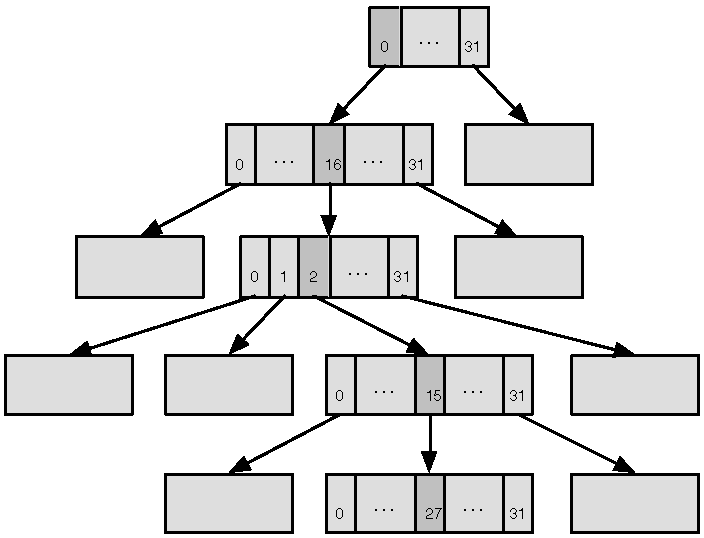
\includegraphics[width=0.5\textwidth]{Figures/Radix_Balanced_index_example}
  \caption{Accessing element at index 526843 in a tree of depth 5. Empty nodes represent collapses subtrees.}
  \label{radix_balanced_index_example}
\end{figure}

%-----------------------------------
\paragraph{Relaxed Radix}
% Explain how to compute them 
% longer, more complex code
% fallback 
When the tree is relaxed it is not possible to know the subindices from index. That is why we keep the sizes array in the unbalanced nodes. This array keeps the accumulated sizes to make the computation of subindices as trivial as possible. The subindex is the same as the first index in the sizes array where $index < sizes[subindex]$. The simplest way to find this subindex is by a linearly scanning the array. 

\begin{lstlisting}[frame=single]
def getSubIndex(sizes: Array[Int], indexInTree: Int): Int = {
  var is = 0
  while (sizes(is) <= indexInTree)
    is += 1
  is
}
\end{lstlisting}

For small arrays (like blocks of size 32) this will take be faster than a binary search because it takes advantage of the cache lines. If we would consider using bigger block sizes it would be better to use a hybrid between binary and linear search.

To traverse the tree down to the leaf where the index is, the subindices are computed from the sizes as long as the tree node is unbalanced. If the node is balanced, then the more efficient radix based method is used from there to the leaf. 


%-----------------------------------
%	SUBSECTION 3
%-----------------------------------

\subsection{Abstractions}
% function calls
% generic code vs specialized code


%----------------------------------------------------------------------------------------
%	SECTION - Displays
%----------------------------------------------------------------------------------------

\section{Displays}
% describe display fields in vector object
% describe the focus field

\begin{figure}[h!]
  \centering
  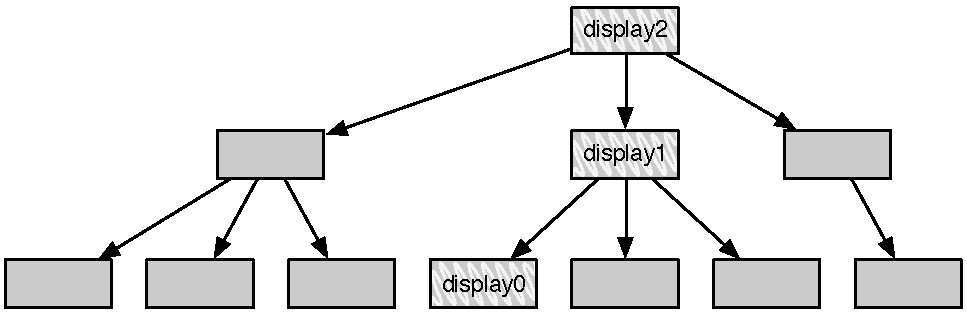
\includegraphics[width=\textwidth]{Figures/Displays}
  \label{Displays}
  \caption{Displays}
\end{figure}

%-----------------------------------
%	SUBSECTION As cache
%-----------------------------------

\subsection{As cache}
% used to access some elements directly from the smaller subtrees (XOR)
% keeping relevant branch for next operations
% operations: all operations that involve the tree structure


%-----------------------------------
%	SUBSECTION  For transient states
%-----------------------------------

\subsection{For transient states}
% transient states are used to amortized operations
% operation: append, prepend, update

\begin{figure}[h!]
  \centering
  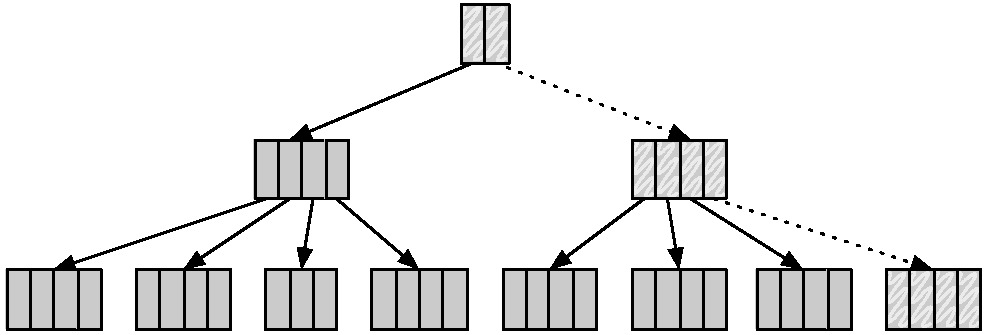
\includegraphics[width=\textwidth]{Figures/Transient_state}
  \label{Transient_state}
  \caption{Radix Balanced Tree Transient state}
\end{figure}


%----------------------------------------------------------------------------------------
%	SECTION - Builder
%----------------------------------------------------------------------------------------

\section{Builder}
% use of mutable tree 
% avoid creation unnecessary arrays



%----------------------------------------------------------------------------------------
%	SECTION - Iterator
%----------------------------------------------------------------------------------------

\section{Iterator}
% efficient tree traversal vs iteration by index
% avoid re-traversing vertically the tree from the root


%----------------------------------------------------------------------------------------
%	SECTION - Relaxing the radix
%----------------------------------------------------------------------------------------

\section{Relaxing the Radix}

%-----------------------------------
%	SUBSECTION Relaxing Displays
%-----------------------------------

\subsection{Relaxing Displays}
% describe fundamental difference in the focus (focused on balanced subtree)
% describe focus start, focus end and focus (focus relaxed)
% describe how fetching elements change

\begin{figure}[h!]
  \centering
  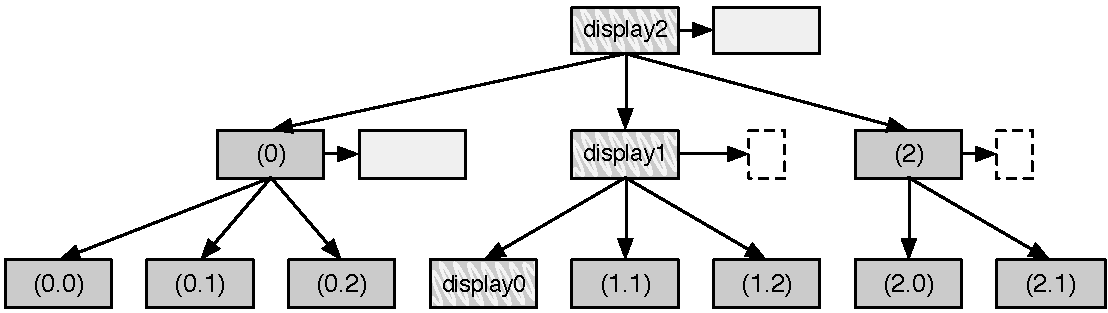
\includegraphics[width=\textwidth]{Figures/Balanced_subtrees}
  \label{Balanced_subtrees}
  \caption{Radix Balanced Tree}
\end{figure}

%-----------------------------------
%	SUBSECTION Displays
%-----------------------------------

\subsection{Relaxing the Builder}
% same base implementation for +=
% addition of accumulator for  ++= 

%-----------------------------------
%	SUBSECTION Displays
%-----------------------------------

\subsection{Relaxing Iterator}
% same implementation within a balanced subtree
% refocus from root to iterate between balanced subtrees



